\begin{question}
\noindent A UI/UX designer is animating a triangular logo icon, $T$, on a design grid before applying two motion effects in sequence.

Triangle $T$ has vertices $A(1,1)$, $B(3,1)$ and $C(1,3)$.

\begin{center}
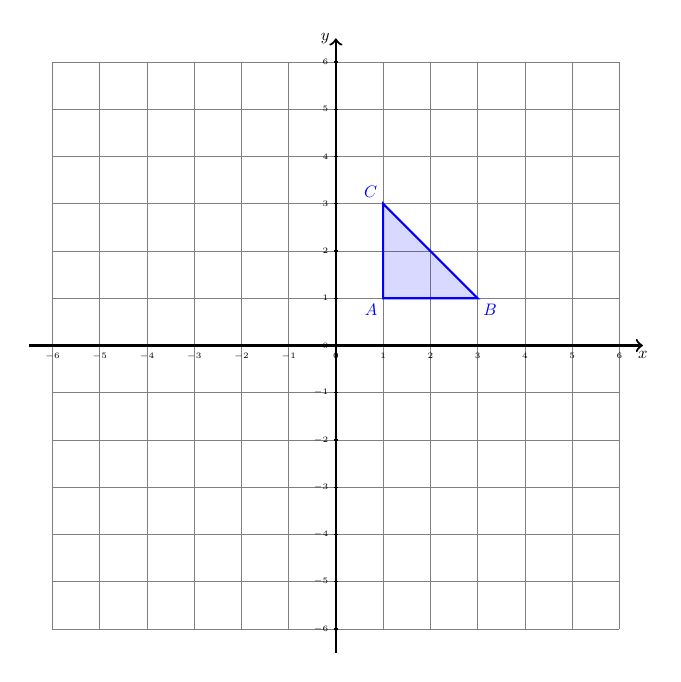
\begin{tikzpicture}[scale=0.6, transform shape]
    \def\axisLimit{6}

    \draw[step=1cm,gray,very thin] (-\axisLimit,-\axisLimit) grid (\axisLimit,\axisLimit);

    \draw[thick,->] (-\axisLimit-0.5,0) -- (\axisLimit+0.5,0) node[anchor=north] {$x$};
    \draw[thick,->] (0,-\axisLimit-0.5) -- (0,\axisLimit+0.5) node[anchor=east] {$y$};

    \foreach \x in {-\axisLimit,...,\axisLimit}
        \draw (\x cm,1pt) -- (\x cm,-1pt) node[anchor=north, font=\tiny] {$\x$};
    \foreach \y in {-\axisLimit,...,\axisLimit}
        \draw (1pt,\y cm) -- (-1pt,\y cm) node[anchor=east, font=\tiny] {$\y$};

    \draw[thick, blue, fill=blue, fill opacity=0.15] (1,1) -- (3,1) -- (1,3) -- cycle;
    \node[blue, below left] at (1,1) {$A$};
    \node[blue, below right] at (3,1) {$B$};
    \node[blue, above left] at (1,3) {$C$};
\end{tikzpicture}
\end{center}

\noindent The design software first applies a rotation of $90^\circ$ clockwise about the origin $O(0,0)$ to triangle $T$, giving triangle $T'$.

\noindent It then reflects triangle $T'$ in the $x$-axis, giving the final animated triangle $T''$.

\begin{enumerate}
    \item[(a)] Find the coordinates of the vertices of triangle $T'$.

    \vspace{4cm}
    \answermarks{2}

    \item[(b)] Find the coordinates of the vertices of triangle $T''$.

    \vspace{3.5cm}
    \answermarks{1}

    \item[(c)] Describe fully the single transformation that maps triangle $T$ directly onto triangle $T''$.

    \vspace{3cm}
    \answerlines{2}{1}
\end{enumerate}
\end{question}
